\section{Discussion and Directions for Future Research}\label{sec:future}


\begin{figure}
  \centering
  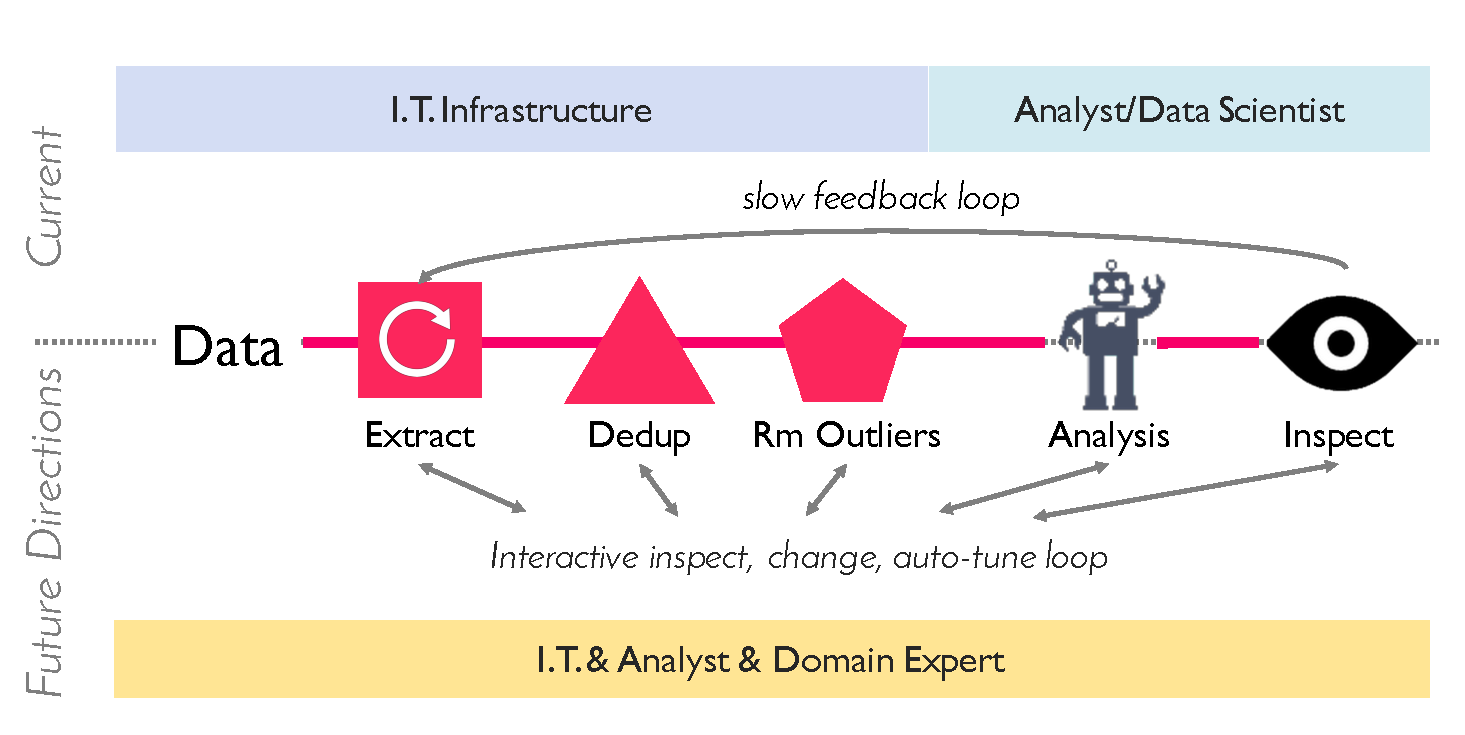
\includegraphics[width=.9\columnwidth]{datafigs/arch}
  \caption{Something}
  \label{f:arch}
\end{figure}

Our survey results highlighted examples in the data cleaning and analysis process that add friction on the iterative data cleaning and analysis process.  The primary finding reiterates the observation that data cleaning is highly contextual---users intimately familiar with the downstream applications are needed to direct the data cleaning process.  In other words, these domain experts are the most important ``humans in the data cleaning loop''.  

Contrary to this understanding, we found that the data cleaning process commonly split across multiple organizations: the IT department performs data cleaning and sends the processed data to application developers and data scientists (top of Figure~\ref{f:arch}).  This separation inhibits the ability to experiment and test different cleaning procedures and tune their parameters---we find that feedback about the data cleaning process is often delayed until the downstream application developer (e.g., visually) inspects the application results.  We believe that these limitations need not exist, and envision a highly interactive data cleaning and analysis process, where {\color{red}{something sexy}} (bottom of Figure~\ref{f:arch}). To this end, we present a series of technical challenges that span HCI and data management to move us towards a more interactive world.

% As highlighted in the top half of Figure~\ref{f:arch}, changes to the cleaning process occur based on observations made at the end of the analysis pipeline.  


\noindent\textbf{Developing High-level Language for Domain Experts:} Data cleaning is an involved process that involves extraction, schema/ontology matching, value imputation, deduplication, and other processes.  In addition, each of these operations encapsulates dozens of specialized algorithms such as machine learning, clustering, or rule-based procedures.  It is both difficult for domain experts to navigate through the zoo of options, and easy for the data cleaners to become married to a particular process---especially when there is a sunk cost.  There is a need for a high level language to describe the data cleaning goals (e.g., providing deduplication examples, descriptions of outliers) that is suitable for domain experts yet usable by the technical experts that are tasked with implementing data cleaning at scale. {\color{red}{more details?}}


\noindent\textbf{Usability and Interactivity:} The value of interactive visual interfaces has been confirmed across numerous domains.  In text extraction, systems such as Wrangler~\cite{} have enabled domain experts to perform complex extraction tasks at scale.  Similarly, systems such as Polaris~\cite{tableau} enable business analysts to perform complex datacube analysis through a visual interface.  Similarly, there is a need to lift a high-level cleaning language into the interactive domain~\cite{joecidr} in order to tighten the feedback loop between the user and cleaning process.

% Often times the domain experts are not techincal experts\footnote{Although our user study population is biased towards technical users, other studies~\cite{kandelsurvey} have shown that data analysts are often non-technical domain experts.}, and there is a need to map the high-level language into the visual interactive domain.  We have seen success from intergrating a domain specific language and visual interactions  in specialized data cleaning domains such as text extraction~\cite{wrangler}.  Similarly agreementmaker work.
% 
% long pipeline from cleaning and output, so insert inspection.  

\noindent\textbf{Application-oriented Cleaning:}  A recurring theme amongst our survey participants was the observation that the data cleaning was driven by the needs of the downstream application.  We found less evidence of data cleaning as a discrete process that happened independently of the application.  The value of application-driven cleaning has potential---recent work such as SampleClean~\cite{} and ActiveClean~\cite{} have found that the cost of data cleaning can be reduced by {\color{red}{an order of magnitude or more}} as compared to an application-independent process.   However these systems have been tailored to specialized use cases (individual aggregation queries and convex models, respectively), and support for more complex sequences of analyses and more complex applications is needed.

\noindent\textbf{Human-Computer Symbiosis:}  Configuration tuning is intimately tied to the data cleaning process and is often manual.  For instance, a developer may modify a parameter values and visually inspecting the downstream results.  Many systems~\cite{} have advocated for automating parts of this process.  For instance, active learning is used as part of crowd-sourced label acquisition~\cite{} to optimize an operation such as deduplication.  Wrangler automatically generates string extraction rules so that the user only needs to pick from a set of options.  Similarly, Tupac~\cite{tupac} performs automatic hyperparameter tuning for machine learning models.   There is similar opportunity to automatically configure other data cleaning operations, as well as propose modifications to the data cleaning workflow itself~\cite{wisteria}.  The ultimate goal is to {\it let experts do what they do best, while machines do the rest}.


\noindent\textbf{Testing and Debugging:} In order to develop automated optimization and tuning procedures, there must be a metric to optimize.  This can be inherently challenging---participants noted that their measure of data cleaning effectiveness was whether or not the downstream process compiled and ran---however the number of compilation errors may not be desirable nor sound.  Thus, methods of introduce metrics throughout the cleaning and analysis pipelines are needed.  For example, by providing a gold dataset of known clean data that the system can compare against.  

Along these lines, as data-cleaning researchers, there is a need for a ``dirtiness'' benchmark analgous to industry standard transaction and analytical data processing benchmarks.  Existing evaluations are often based on synthetically generated errors and are susceptible to overfitting to synthetic cases or specialized types of errors evaluated in isolation.  

%Such a benchmark needs to support cases when there is and is not a ground truth dataset.

\noindent\textbf{Combating Overfitting:} Along the lines of testing and debugging, we find evidence of overfitting the data cleaning procedures to the specific instance of the downstream applicationi.  For instance, {\color{red}{EXAMPLE}}.  This can lead to overly complex, brittle data cleaning pipelines that are hard to share with other applications and may not apply to future evolutions of the application.  APPLY SANJAY

In summary, we are in the early days of highly interactive data cleaning and preparation and we are optimistic about the improvement that can be made by bringing user interactivity into the process.


\if{0}
 
* A language or languages for data cleaning.  An operation, such as deduplication involves a large number of possible algorithms or sytems techinques, ranging from crowdsourced solsutions(REF Anhai), machine learning-based fuzzy matching(REF).  It is often easier for a user to provide correct results rather than.
* Be careful about survey biased towards technical people, not those that use GUIs. 
* Usability: Tied with the language are a set of interactions to match the language operations (REF joe’s CIDR paper).  This is admittedly an amorpheous topic.  (REF agreementmaker work)
* Goal oriented cleaning.  General data cleaning is rarely needed, and pay-as-you-go solutions(REF data spaces) are needed in most applications.   This begs the qusetion for hminimizing expert involvement.   Solutions such as sampleclean are oriented towards specializing the human effort towards porudictive tasks that maximize the cleaning for a particular application.  
* Automation. 
    * Hyperparameter tuning, however visual inspection by manually tuning each or combinations of parameters is both slow and and error-prone.  Automated hyperparemeter tuning (REF evan)
    * String value munging, either deduplication, extraction, fixes.  Existing tools are often not sufficient and user intervention (REF Wrangler) is necessary.  However even in this settings, ways to generate suggestions and show them is better than users picking operations to perform.
    * active learning is used, but only for crowd workers that fit inside an operator good progress folks.
    * Opporutinity let the expert be the human in the loop.  The data analyst IS the human in the loop.
    * Let humans do what they do best, machines to the rest.
* Testing and debugging cleaning.  Data cleaning does not live within a vacuum.  It is often motivated by a set of desired applications, and .  How can it be tested?  For example, what effects will introducing or modiying a data cleaning procedure have on the rest of the dataset, or the downstream application?  For example, in our survey several respondents noted that their evaluation was based on whether the downstream applicaiton compiles or not.
    * Reference Self eval idea.  long pipeline from cleaning and output, so insert inspection.  
    * Reference benchmarking work and systematic ways to evaluate the efficacy of an approach when there is ground truth and when there is no ground truth.
* (SANJAY) Overfitting and sharing.   It is easy to overfit the data cleaning to the intricacies of a particular application and the data for that application.  Although this is easy to do, it makes it difficult to share and re-use data cleaning procedures for similar tasks in the future, or share within an organization.  In these cases, tools to help prevent overfitting, similar to regularization in machine learning, are needed to help generalize data cleaning workflows into reusable components.  High level scripting languages can help in this regard, but automated tools are also needed.




* Here’s a general system/interactive loop that is pie in the sky that would workfor the 99% cases.
    * Data cleaning is user and context dependent.  So much relies on the developer’s, or downstream user's expert knowledge that interactive solutions are needed.    
    * In fact, in some cases, the data cleaning process is divorced from the users using the data cleaning, which is surprising given the context-sensitive nature.
    * trying cleaning procedures, algorithms, tuning parameters out, and evaluating the results through visual inspection of computed metrics, or the cleaned data
    * Needs highly interactive systems, and often visual systems for domain experts
    * Figure 1 shows a highlevel loop
    * Only when combined into a single system does it make sense
    * This motivates a set of interesting technical problems that we outline below.

\fi
